\chapter{Caso de estudio: QVTWSInvoker}
\label{Caso de estudio: QVTWSInvoker}

En este capítulo se presenta un caso de estudio que plantea el uso de Web Services (WS) seleccionados automáticamente en la invocación de aplicaciones externas al Workflow Management System (WFMS), a través de su aplicación en el marco de las tareas involucradas en el proceso de desarrollo de software denominado QVTWSInvoker.


\section{Descripción general de la herramienta}

En virtud de lograr el cumplimiento de los objetivos enunciados en la sección 1.2 una gran cantidad de factores han sido tenidos en cuenta para finalmente llegar a una solución acorde a las expectativas.\\
QVTWSInvoker utiliza una plantilla genéricas de entrada. Consiste de un conjunto de parámetros que son los encargados de transportar los requerimientos del usuario a la herramienta. Y dado que este usuario será en reiteradas ocasiones un WFMS, el conjunto de parámetros ha sido planteado simple y estándar. Esta plantilla está formada por los siguientes atributos: tipo de WS, nombres y descripción de la operación a ejecutar con sus respectivos parámetros (valores para los cuales se deseen obtener los resultados correspondientes). Esta parametrización le posibilitará a la herramienta acceder de manera estándar a los requerimientos del sistema siempre de una misma forma, para luego comenzar el proceso de búsqueda con los criterios y filtros correspondientes.\\
La salida de la herramienta se imprime en un texto simple. Luego de la salida se le pide al usuario que especifique si está satisfecho con el resultado del WS.\\
Es importante destacar, que la herramienta provee al usuario las diferentes alternativas que desee en cuanto al tipo de WS y además, le da la posibilidad de proveer información para actualizar las características de calidad (QoS) que implementa dicho WS. 

\section{Proceso de selección de WS's}

El proceso de selección de WS's con sus respectivas ejecuciones, consiste en la transformación de los requerimientos del usuario en una instancia salida. Este proceso lo realiza QVTWSinvoker implementando los mecanismos descritos en los capítulos \ref{Mecanismo de selección de Web Services} y \ref{Caso de estudio: QVTWSInvoker} que se describe en los siguientes puntos:\\

\textbf{Fase 1: Obtención de Parámetros}\\

En esta fase la herramienta obtiene desde la plantilla de entrada los parámetros, los números del mensaje de entrada se corresponden a estos parámetros. Ellos significan: 1 = tipo del WS; 2 = nombre de las operaciones; 3 = descripción ; 4 = cantidad y tipo de los parámetros; (Ver figura \ref{fig:Plantilla de entrada de solicitud de usuario})\\

\begin{figure}[!h] 
	\begin{center}
		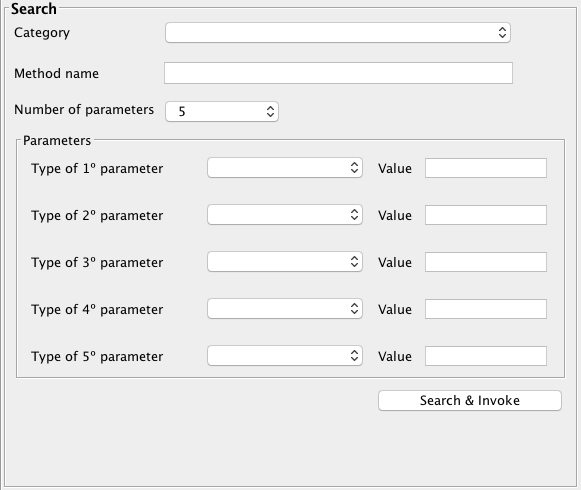
\includegraphics [scale=0.60]{imagenes/Plantilla_de_entrada_de_solicitud_de_usuario.png}
	\end{center}
	\caption{Plantilla de entrada de solicitud de usuario}
	\label{fig:Plantilla de entrada de solicitud de usuario}
\end{figure} 

\textbf{Fase 2: Obtención de WS's de la base de datos}\\

La base de datos contiene los WS's conocidos por la herramienta. Se compone de la información los WSDL y las QoS.  En esta fase la herramienta, en base al tipo ingresadas por el usuario en la plantilla de entrada y las QoS , obtiene de la base de datos la lista de descripciones de los WS's ordenada por valor de ponderación de las QoS (mecanismo de calificación descrito en el capítulo \ref{Mecanismo de selección de Web Services}). 

\lstinputlisting[ firstline=113, lastline=129,caption={Método que obtiene de la base de datos la lista de descripciones},label={code:Método que obtiene de la base de datos la lista de descripciones}]{../QVTWSInvoker/src/tesis/crud/CategoryCRUD.java}

\lstinputlisting[ firstline=8, lastline=15,caption={Método comparador para ordenar la cola},label={code:Método comparador para ordenar la cola}]{../QVTWSInvoker/src/tesis/utils/WsdlComparator.java}


\textbf{Fase 3: Transformaciones y Filtro por nombre, descripción y parámetros de la operación}\\

A partir del conjunto de WS's generado en la fase previa, la herramienta procede a transformarlos siguiendo el mecanismo descripto en el cap 5 y filtrarlas teniendo en cuenta nombre, descripción y parámetros de la operación que se especificaron en la plantilla de entrada.\\	

\textbf{Fase 4. Ejecución de WS's}\\

En la ejecución de WS's se selecciona el primer WS del conjunto. Una ejecución consiste en la invocación del WS con los parámetros que el usuario pasa en la plantilla de entrada. Si el resultado de esta ejecución es exitoso, la herramienta retorna la salida cuyos datos son los obtenidos de la ejecución.\\
Una ejecución se considera exitosa cuando se muestran  los datos obtenidos de la invocación del WS. Si la ejecución no es exitosa se toma el siguiente WS y se repite esta fase.


\lstinputlisting[ firstline=215, lastline=244,caption={Invocación al mejor WS},label={code:Invocación al mejor WS}]{../QVTWSInvoker/src/tesis/controllers/InvokerController.java}


\textbf{Fase 5: Calificación del WS's}\\

Esta última fase le solicita al usuario información respecto a la calidad del servicio preguntándole si la salida ha satisfecho sus necesidades. Luego de que compute la respuesta, esta se utiliza para calcular la reputación del servicio.


\begin{figure}[!h] 
	\begin{center}
		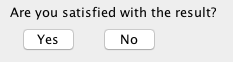
\includegraphics [scale=1.00]{imagenes/Interfaz_de_usuario_satisfecho.png}
	\end{center}
	\caption{Interfaz de usuario correspondiente a la fase 5}
	\label{fig:Interfaz de usuario correspondiente a la fase 5}
\end{figure} 


\lstinputlisting[ firstline=76, lastline=92,caption={Controlador que captura la respuesta del usuario},label={code:Controlador que captura la respuesta del usuario}]{../QVTWSInvoker/src/tesis/controllers/InvokerController.java}

\lstinputlisting[ firstline=123, lastline=148,caption={Método que edita la reputación del WS en la base de datos},label={code:Método que edita la reputación del WS en la base de datos}]{../QVTWSInvoker/src/tesis/crud/WsdlCRUD.java}

\section{Diseño de la herramienta}

\subsection{Arquitectura general}

\begin{figure}[!h] 
	\begin{center}
		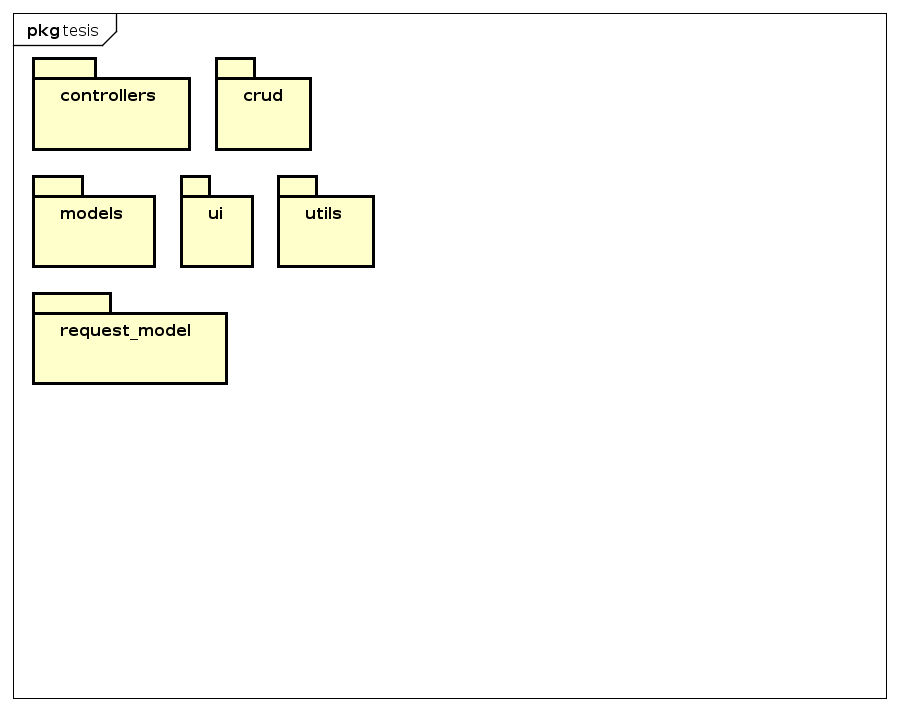
\includegraphics [scale=0.70]{imagenes/paquetes.png}
	\end{center}
	\caption{Paquetes del proyecto}
	\label{fig:Paquetes del proyecto}
\end{figure} 

El programa fue construido con el patrón modelo–vista–controlador (MVC), el cual separa los datos y la lógica de negocio de una aplicación de la interfaz de usuario y el módulo encargado de gestionar los eventos y las comunicaciones . A continuación se describen los paquetes de la figura:

\begin{itemize}
	\item \textbf{controllers:} Clases que gestionan los eventos y las comunicaciones entre los modelos y la interfaz de usuario.
	\item \textbf{crud:} Clases que gestionan las altas, bajas y modificaciones de los modelos.
	\item \textbf{models:} Cases que representan los modelos de categoría y wsdl necesarias con el uso de la librería Active JDBC. 
	\item \textbf{ui:} Clases que implementan la interfaz de usuario.
	\item \textbf{utils:} Clases de utilidad en el sistema.
	\item \textbf{request\_model:} Contiene el modelo de los requisitos del usuario.
\end{itemize}

MVC propone la construcción de tres componentes distintos que son el modelo, la vista y el controlador, es decir, por un lado define componentes para la representación de la información, y por otro lado para la interacción del usuario. Por ejemplo, el módulo de gestión de categorías está diseñado de la forma en que se observa en la figura \ref{fig:Paquete controllers ejemplo category}\\

 \begin{figure}[H]  
 	\begin{center}
 		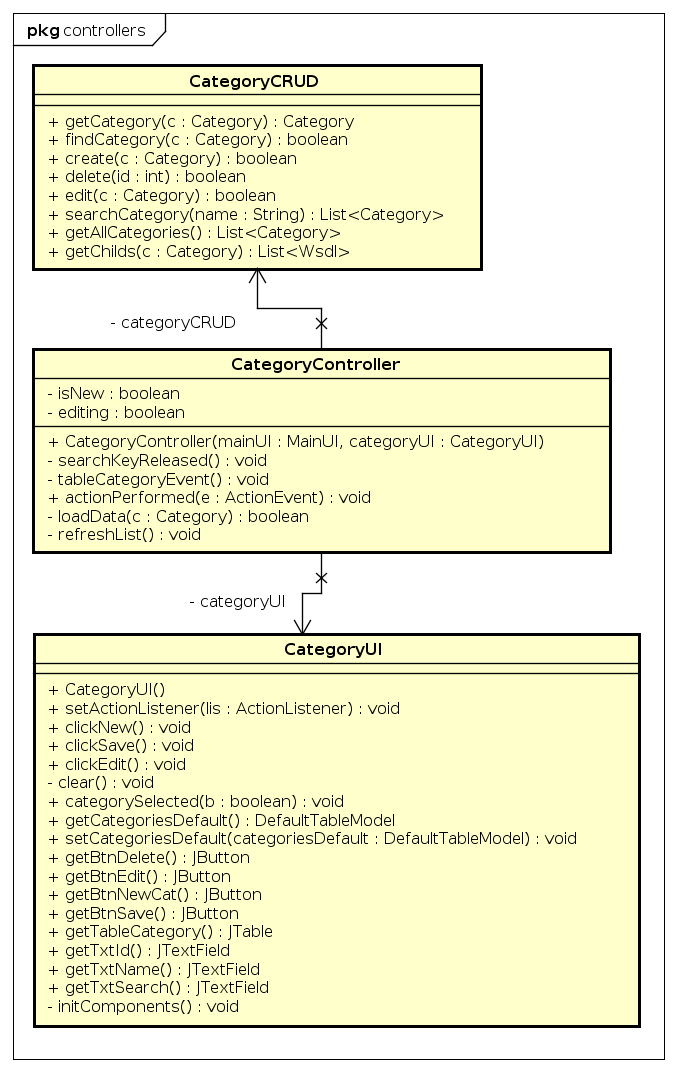
\includegraphics [scale=0.80]{imagenes/paquete_controllers.png}
 	\end{center}
 	\caption{Paquete controllers ejemplo Category}
 	\label{fig:Paquete controllers ejemplo category}
 \end{figure} 


 Claramente se puede observar que CategoryUI implementa la interfaz de usuario, CategoryCrud el modelo y CategoryController el controlador.\\
 
 El diagrama de clase para WsdlCrud es similar al de CategoryCrud, solo difiere en los atributos\\
 
 El diagrama de clases de diseño de la herramienta QVTWSInvoker ilustrado en la figura \ref{fig:Diagrama de clases general}, muestra cómo se relacionan las principales clases.\\

  \begin{figure}[H] 
  	\begin{center}
  		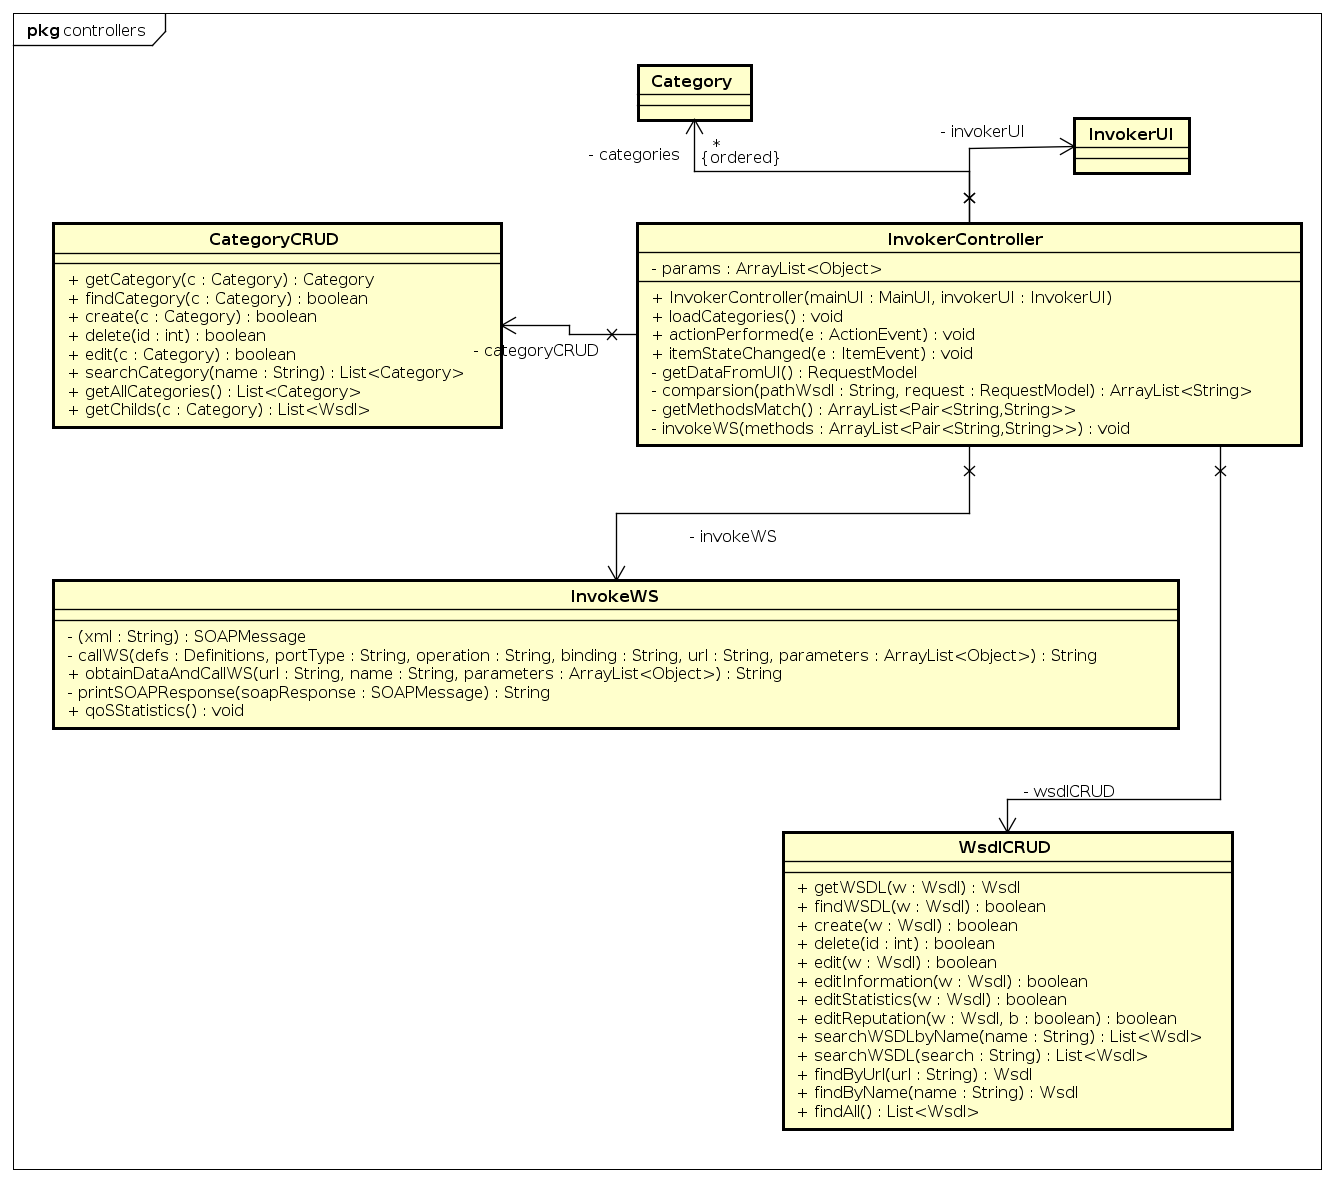
\includegraphics [scale=0.45]{imagenes/diagrama_clases_general.png}
  	\end{center}
  	\caption{Diagrama de clases general}
  	\label{fig:Diagrama de clases general}
  \end{figure}


   En este diagrama (figura \ref{fig:Diagrama de clases general}) se puede observar que las clases InvokeWS y InvokerController son las más importantes. \\
  La clase InvokeController es la encargada de obtener la petición desde la interfaz de usuario, para luego obtener los wsdl de la categoría elegida a través del CRUD wsdlCRUD. Una vez que se tienen los wsdl y se le realiza la transformación QVT y obtención del mejor método explicado en el capítulo anterior, se pasa a la etapa de ejecución del método del wsdl. Para ello, se utiliza la clase InvokeWS,\\
  esta fue construida con la ayuda de la librería SOA\_Distribution la cual permite automatizar la invocación a un método SOAP, una vez invocado, el resultado es mostrado por la interfaz de usuario a través del controlador InvokerController.
  
  \subsection{Modelo de Persistencia}
  
  El diagrama de clases persistentes de la herramienta QVTWSInvoker se muestra en la figura. Este conjunto de clases es responsable de almacenar la información de los WS's por cada ejecución. (ver figura \ref{fig:Modelo persistente de la herramienta QVTWSInvoker})\\
  
  \begin{figure}[!h] 
  	\begin{center}
  		\includegraphics [scale=0.45]{imagenes/modelo_persistente.png}
  	\end{center}
  	\caption{Modelo persistente de la herramienta QVTWSInvoker}
  	\label{fig:Modelo persistente de la herramienta QVTWSInvoker}
  \end{figure}
  
  A continuación se describen las tablas de la figura:\\
  
  La tabla Category representa las categorías de los WS'ss, tiene un id único que funciona como clave y un nombre, por su parte, la tabla Wsdl se encarga de mantener la información sintáctica básica de cualquier wsdl: identificador, nombre, url y categoría, además de guardar la información respecto a su calidad de servicio (reputación, tiempo de respuesta y disponibilidad).\\
  
  
\section{Herramientas utilizadas}
  
En esta sección describiremos las diferentes herramientas y tecnología utilizadas a lo largo de la construcción de este trabajo:\\

\textbf{NetBeans y Eclipse IDE} son entornos de desarrollo herramientas para que los programadores puedan escribir, compilar, depurar y ejecutar programas fácilmente.\\ 		

\textbf{Java 1.8} es un lenguaje de programación orientado a objetos que pertenece a la empresa Sun Microsystems. Entre sus características podemos nombrar: simple, distribuido, robusto, portable, interpretado, multitareas. Se utilizó como lenguaje de programación base dentro de la herramienta NetBeans.\\

\textbf{GlassFish} es un servidor de aplicaciones de software libre desarrollado por Sun Microsystems, que implementa las tecnologías definidas en la plataforma Java EE y permite ejecutar aplicaciones que siguen esta especificación. Es gratuito y de código libre, se distribuye bajo un licenciamiento dual a través de la licencia CDDL y la GNU GPL.\\

\textbf{H2} es un sistema administrador de bases de datos relacionales programado en Java. Una de las características más importantes de H2 es que se puede integrar completamente en aplicaciones Java y acceder a la base de datos lanzando SQL directamente, sin tener que pasar por una conexión a través de sockets. Está disponible como software de código libre bajo la Licencia Pública de Mozilla o la Eclipse Public License.\\

\textbf{Eclipse Modeling Tools} contiene marcos de trabajos y herramientas para trabajar con modelos: Un modelador gráfico de Ecore, utilidad de generación de código Java para aplicaciones RCP y el marco de trabajo EMF, soporte para comparación de modelos, para esquemas XSD, OCL y modeladores gráficos en tiempo de ejecución.    